%  LaTeX support: latex@mdpi.com 
%  For support, please attach all files needed for compiling as well as the log file, and specify your operating system, LaTeX version, and LaTeX editor.

%=================================================================
\documentclass[energies,article,submit,pdftex,moreauthors]{Definitions/mdpi} 
% For posting an early version of this manuscript as a preprint, you may use "preprints" as the journal and change "submit" to "accept". The document class line would be, e.g., \documentclass[preprints,article,accept,moreauthors,pdftex]{mdpi}. This is especially recommended for submission to arXiv, where line numbers should be removed before posting. For preprints.org, the editorial staff will make this change immediately prior to posting.

%--------------------
% Class Options:
%--------------------
%----------
% journal
%----------
% Choose between the following MDPI journals:
% acoustics, actuators, addictions, admsci, adolescents, aerospace, agriculture, agriengineering, agronomy, ai, algorithms, allergies, alloys, analytica, animals, antibiotics, antibodies, antioxidants, applbiosci, appliedchem, appliedmath, applmech, applmicrobiol, applnano, applsci, aquacj, architecture, arts, asc, asi, astronomy, atmosphere, atoms, audiolres, automation, axioms, bacteria, batteries, bdcc, behavsci, beverages, biochem, bioengineering, biologics, biology, biomass, biomechanics, biomed, biomedicines, biomedinformatics, biomimetics, biomolecules, biophysica, biosensors, biotech, birds, bloods, blsf, brainsci, breath, buildings, businesses, cancers, carbon, cardiogenetics, catalysts, cells, ceramics, challenges, chemengineering, chemistry, chemosensors, chemproc, children, chips, cimb, civileng, cleantechnol, climate, clinpract, clockssleep, cmd, coasts, coatings, colloids, colorants, commodities, compounds, computation, computers, condensedmatter, conservation, constrmater, cosmetics, covid, crops, cryptography, crystals, csmf, ctn, curroncol, currophthalmol, cyber, dairy, data, dentistry, dermato, dermatopathology, designs, diabetology, diagnostics, dietetics, digital, disabilities, diseases, diversity, dna, drones, dynamics, earth, ebj, ecologies, econometrics, economies, education, ejihpe, electricity, electrochem, electronicmat, electronics, encyclopedia, endocrines, energies, eng, engproc, ent, entomology, entropy, environments, environsciproc, epidemiologia, epigenomes, est, fermentation, fibers, fintech, fire, fishes, fluids, foods, forecasting, forensicsci, forests, foundations, fractalfract, fuels, futureinternet, futureparasites, futurepharmacol, futurephys, futuretransp, galaxies, games, gases, gastroent, gastrointestdisord, gels, genealogy, genes, geographies, geohazards, geomatics, geosciences, geotechnics, geriatrics, hazardousmatters, healthcare, hearts, hemato, heritage, highthroughput, histories, horticulturae, humanities, humans, hydrobiology, hydrogen, hydrology, hygiene, idr, ijerph, ijfs, ijgi, ijms, ijns, ijtm, ijtpp, immuno, informatics, information, infrastructures, inorganics, insects, instruments, inventions, iot, j, jal, jcdd, jcm, jcp, jcs, jdb, jeta, jfb, jfmk, jimaging, jintelligence, jlpea, jmmp, jmp, jmse, jne, jnt, jof, joitmc, jor, journalmedia, jox, jpm, jrfm, jsan, jtaer, jzbg, kidney, kidneydial, knowledge, land, languages, laws, life, liquids, literature, livers, logics, logistics, lubricants, lymphatics, machines, macromol, magnetism, magnetochemistry, make, marinedrugs, materials, materproc, mathematics, mca, measurements, medicina, medicines, medsci, membranes, merits, metabolites, metals, meteorology, methane, metrology, micro, microarrays, microbiolres, micromachines, microorganisms, microplastics, minerals, mining, modelling, molbank, molecules, mps, msf, mti, muscles, nanoenergyadv, nanomanufacturing, nanomaterials, ncrna, network, neuroglia, neurolint, neurosci, nitrogen, notspecified, nri, nursrep, nutraceuticals, nutrients, obesities, oceans, ohbm, onco, oncopathology, optics, oral, organics, organoids, osteology, oxygen, parasites, parasitologia, particles, pathogens, pathophysiology, pediatrrep, pharmaceuticals, pharmaceutics, pharmacoepidemiology, pharmacy, philosophies, photochem, photonics, phycology, physchem, physics, physiologia, plants, plasma, pollutants, polymers, polysaccharides, poultry, powders, preprints, proceedings, processes, prosthesis, proteomes, psf, psych, psychiatryint, psychoactives, publications, quantumrep, quaternary, qubs, radiation, reactions, recycling, regeneration, religions, remotesensing, reports, reprodmed, resources, rheumato, risks, robotics, ruminants, safety, sci, scipharm, seeds, sensors, separations, sexes, signals, sinusitis, skins, smartcities, sna, societies, socsci, software, soilsystems, solar, solids, sports, standards, stats, stresses, surfaces, surgeries, suschem, sustainability, symmetry, synbio, systems, taxonomy, technologies, telecom, test, textiles, thalassrep, thermo, tomography, tourismhosp, toxics, toxins, transplantology, transportation, traumacare, traumas, tropicalmed, universe, urbansci, uro, vaccines, vehicles, venereology, vetsci, vibration, viruses, vision, waste, water, wem, wevj, wind, women, world, youth, zoonoticdis 

%---------
% article
%---------
% The default type of manuscript is "article", but can be replaced by: 
% abstract, addendum, article, book, bookreview, briefreport, casereport, comment, commentary, communication, conferenceproceedings, correction, conferencereport, entry, expressionofconcern, extendedabstract, datadescriptor, editorial, essay, erratum, hypothesis, interestingimage, obituary, opinion, projectreport, reply, retraction, review, perspective, protocol, shortnote, studyprotocol, systematicreview, supfile, technicalnote, viewpoint, guidelines, registeredreport, tutorial
% supfile = supplementary materials

%----------
% submit
%----------
% The class option "submit" will be changed to "accept" by the Editorial Office when the paper is accepted. This will only make changes to the frontpage (e.g., the logo of the journal will get visible), the headings, and the copyright information. Also, line numbering will be removed. Journal info and pagination for accepted papers will also be assigned by the Editorial Office.

%------------------
% moreauthors
%------------------
% If there is only one author the class option oneauthor should be used. Otherwise use the class option moreauthors.

%---------
% pdftex
%---------
% The option pdftex is for use with pdfLaTeX. If eps figures are used, remove the option pdftex and use LaTeX and dvi2pdf.

%=================================================================
% MDPI internal commands
\firstpage{1} 
\makeatletter 
\setcounter{page}{\@firstpage} 
\makeatother
\pubvolume{1}
\issuenum{1}
\articlenumber{0}
\pubyear{2022}
\copyrightyear{2022}
%\externaleditor{Academic Editor: Firstname Lastname}
\datereceived{} 
%\daterevised{} % Only for the journal Acoustics
\dateaccepted{} 
\datepublished{} 
%\datecorrected{} % Corrected papers include a "Corrected: XXX" date in the original paper.
%\dateretracted{} % Corrected papers include a "Retracted: XXX" date in the original paper.
\hreflink{https://doi.org/} % If needed use \linebreak
%\doinum{}
%------------------------------------------------------------------
% The following line should be uncommented if the LaTeX file is uploaded to arXiv.org
%\pdfoutput=1

%=================================================================
% Add packages and commands here. The following packages are loaded in our class file: fontenc, inputenc, calc, indentfirst, fancyhdr, graphicx, epstopdf, lastpage, ifthen, lineno, float, amsmath, setspace, enumitem, mathpazo, booktabs, titlesec, etoolbox, tabto, xcolor, soul, multirow, microtype, tikz, totcount, changepage, attrib, upgreek, cleveref, amsthm, hyphenat, natbib, hyperref, footmisc, url, geometry, newfloat, caption

%=================================================================
%% Please use the following mathematics environments: Theorem, Lemma, Corollary, Proposition, Characterization, Property, Problem, Example, ExamplesandDefinitions, Hypothesis, Remark, Definition, Notation, Assumption
%% For proofs, please use the proof environment (the amsthm package is loaded by the MDPI class).

%=================================================================
% Full title of the paper (Capitalized)
\Title{Functional Logistic Regression for Motor Fault Classification Using Acoustic Data in Frequency Domain}

% MDPI internal command: Title for citation in the left column
\TitleCitation{Functional Logistic Regression for Motor Fault Classification Using Acoustic Data in Frequency Domain}

% Author Orchid ID: enter ID or remove command
\newcommand{\orcidauthorA}{0000-0003-3313-581X} % Add \orcidA{} behind the author's name
%\newcommand{\orcidauthorB}{0000-0000-0000-000X} % Add \orcidB{} behind the author's name

% Authors, for the paper (add full first names)
\Author{Jakub Poręba, Jerzy Baranowski \orcidA{}}

%\longauthorlist{yes}

% MDPI internal command: Authors, for metadata in PDF
\AuthorNames{Jakub Poręba, Jerzy Baranowski}

% MDPI internal command: Authors, for citation in the left column
\AuthorCitation{Poręba, J.; Baranowski, J.}
% If this is a Chicago style journal: Lastname, Firstname, Firstname Lastname, and Firstname Lastname.

% Affiliations / Addresses (Add [1] after \address if there is only one affiliation.)
\address{%
AGH University of Science \& Technology; e-mail@e-mail.com, jb@agh.edu.pl}


% Contact information of the corresponding author
\corres{Correspondence: jb@agh.edu.pl;} 

% Current address and/or shared authorship

% The commands \thirdnote{} till \eighthnote{} are available for further notes

%\simplesumm{} % Simple summary

%\conference{} % An extended version of a conference paper

% Abstract (Do not insert blank lines, i.e. \\) 
\abstract{}

% Keywords
\keyword{keyword 1; keyword 2; keyword 3 (List three to ten pertinent keywords specific to the article; yet reasonably common within the subject discipline.)} 

% The fields PACS, MSC, and JEL may be left empty or commented out if not applicable
%\PACS{J0101}
%\MSC{}
%\JEL{}

%%%%%%%%%%%%%%%%%%%%%%%%%%%%%%%%%%%%%%%%%%
% Only for the journal Diversity
%\LSID{\url{http://}}

%%%%%%%%%%%%%%%%%%%%%%%%%%%%%%%%%%%%%%%%%%
% Only for the journal Applied Sciences
%\featuredapplication{Authors are encouraged to provide a concise description of the specific application or a potential application of the work. This section is not mandatory.}
%%%%%%%%%%%%%%%%%%%%%%%%%%%%%%%%%%%%%%%%%%

%%%%%%%%%%%%%%%%%%%%%%%%%%%%%%%%%%%%%%%%%%
% Only for the journal Data
%\dataset{DOI number or link to the deposited data set if the data set is published separately. If the data set shall be published as a supplement to this paper, this field will be filled by the journal editors. In this case, please submit the data set as a supplement.}
%\datasetlicense{License under which the data set is made available (CC0, CC-BY, CC-BY-SA, CC-BY-NC, etc.)}

%%%%%%%%%%%%%%%%%%%%%%%%%%%%%%%%%%%%%%%%%%
% Only for the journal Toxins
%\keycontribution{The breakthroughs or highlights of the manuscript. Authors can write one or two sentences to describe the most important part of the paper.}

%%%%%%%%%%%%%%%%%%%%%%%%%%%%%%%%%%%%%%%%%%
% Only for the journal Encyclopedia
%\encyclopediadef{For entry manuscripts only: please provide a brief overview of the entry title instead of an abstract.}

%%%%%%%%%%%%%%%%%%%%%%%%%%%%%%%%%%%%%%%%%%
\begin{document}

%%%%%%%%%%%%%%%%%%%%%%%%%%%%%%%%%%%%%%%%%%
% \section{How to Use this Template}

% The template details the sections that can be used in a manuscript. Note that the order and names of article sections may differ from the requirements of the journal (e.g., the positioning of the Materials and Methods section). Please check the instructions on the authors' page of the journal to verify the correct order and names. For any questions, please contact the editorial office of the journal or support@mdpi.com. For LaTeX-related questions please contact latex@mdpi.com.%\endnote{This is an endnote.} % To use endnotes, please un-comment \printendnotes below (before References). Only journal Laws uses \footnote.

% The order of the section titles is: Introduction, Materials and Methods, Results, Discussion, Conclusions for these journals: aerospace,algorithms,antibodies,antioxidants,atmosphere,axioms,biomedicines,carbon,crystals,designs,diagnostics,environments,fermentation,fluids,forests,fractalfract,informatics,information,inventions,jfmk,jrfm,lubricants,neonatalscreening,neuroglia,particles,pharmaceutics,polymers,processes,technologies,viruses,vision


\section{Introduction}

Functional data is the way of data interpretation where each subject is considered as a continuous curve. This field became more popular in recent years in various fields of science, for example biology and economics. Hence, with the rapid popularity grow, new sub-field of statistics appeared, called functional data analysis (FDA). Due to high dimensionality of considered data, many approaches of FDA are based on basis expansions and principle components analysis. Another part of FDA, used for example in case of time series analysis, is data classification. In this case, methods analogical to existing in traditional statistics can be used. 

Many researchers have already presented several methods of FDA, including funtional logistic regression \cite{ramsay-logreg, ramsay-logreg2, ramsay1982data} and functional principal component analysis \cite{besse-pca, pezzulini-pca}. Mousavi and Sørensen made great comparison of several methods of functional logistic regression \cite{logreg-comparison}, and Berrendero et al. described possible issues and problems with implementation \cite{logreg-issues}.

In this paper the general approach and proposed implementation of time series data classification using functional logistic regression both in binary and multiclass variants is presented. To handle the dimensionality of data, voice recordings of commutator motors described in \cite{ref-motors}, B-spline functions of parametrized order are used.

%%%%%%%%%%%%%%%%%%%%%%%%%%%%%%%%%%%%%%%%%%

\section{Methods and Materials}
\subsection{Functional data analysis}
Functional data analysis is the way of analysis where data is in the form of functions, images or other more general objects, even with infinite dimension. Historically, first approach of using such a way of analysis was written down by Grenander \cite{grenander1950stochastic} and Rao \cite{rao1958some} in 1950s, but the term "functional data analysis" was firstly introduced and described by Ramsay et. al. \cite{ramsay-logreg, ramsay-logreg2, ramsay1982data}. Great modern review of this field of stochastics and statiscics is made by Wang et. al. \cite{wang2016functional}. As FDA is a collection of statistical techniques for functions, it tries to answer many questions similar to ones existing in classic statistics and data analysis, like "what is the main way in which one curve differs from another". The big advantage of FDA is, that instead of considering just the given data and curves as they are, their rates of changes (or derivatives) can be described as well.

As functional data is a general term, it can cover several real data examples collected in several different ways. One of approaches is to use series of samples (if ordered in time, then it will be time series) and interpolate the space between particular samples. This way functional data analysis deals with the finite resolution of physical devices. However, data can be stored in other ways and can be of shape completely different than one-dimensional series. One example is to use principal component analysis on complex, high-resolution spectroscopic surveys \cite{Patil_2022}. Neural networks can be fed with functional data as well \cite{rossi2005representation}.

While introducing FDA, Ramsay showed a difference between a \emph{standard} and \emph{functional analytic view} of data and the generalization of vectors \cite{ramsay1982data}. All elements of finite dimensional vectors can be represented as weighted sums of a finite number \emph{p} of \emph{basis vectors} or, in functional world, \emph{basis functions}. Basis function is a tool which helps with producing a complex functions $ f(t) $ by stacking $ k $ more simple ones, $ \phi_k(t) $, which Ramsay calls \emph{mathematical Lego}. Thus, the linear combination of basis functions can be described:

\begin{linenomath}
\begin{equation}
f(x) = a_1 \phi_1(t) + a_2 \phi_2(t) + ... + a_k \phi_k(t)
\end{equation}
\end{linenomath}

Second very important concept in functional data analysis are \emph{spline functions} (splines). These functions are formed by joining polynomials together at fixed points called \emph{knots}, forming together an approximation of origin function $ f(t) $. Assume there is function $ f(t) $ in $ {\Bbb R} $ and there is a need to approximate its values within interval limited from both sides by lower boundary $ t_L $ and upper boundary $ t_U $. In such interval, there can be made $ L+1 $ sub-intervals $ \xi_l $ separated by $ L $ knots. In each knot two polynomials must join together smoothly, so the derivative (for all degrees up to one less than the polynomials degree) of connected splines exists.

\begin{figure}[H]
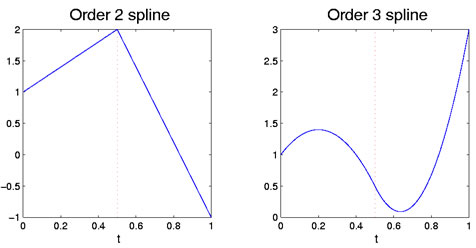
\includegraphics[width=10.5 cm]{images/splines_example.png}
\caption{Sample spline functions of second (left, linear) and third (right, quadratic) orders with knots at 0.5 (example based on \href{https://www.psych.mcgill.ca/misc/fda/ex-basis-b1.html}{Ramsay's introduction into FDA}.)}
\end{figure}
\unskip
\vspace{5mm}

The figure above presents two examples of spline functions, for second and third order, with one knot joining together two splines. If each polynomial is of first degree (straight line, order 2 splines), then in knots derivatives up to degree 0 must match, so in this example polynomials must have the same values at connecting points. As the second spline function has already one point defined by knot and previous spline, then it looses only one degree of freedom instead of two. Similar situation is with spline functions of third order. They derivatives at knot for two connecting second degree polynomials matches up to first degree. The second spline has limited points of freedom to just one because of the constraints at connecting point: value and the slope described by the derivative of first polynomial at this point.

\subsection{Binary Logistic Regression}
Logistic regression is a widely used classification concept. It is mainly applied, and was originally described, for binary problems, however its multiclass version (Softmax) is also well known. As a statistical method, logistic regression allows to measure how several independent variables $ x_1, x_2, ...,  x_k $ affect binary dependent variable $Y$, for example what is the influence of time spent on watching TV series and learning (two independent variables) on the exam results (if passed or not). 

In typical mathematical problems both dependent and independent variables are continuous. If so, the relation of linear regression can be established:
\begin{linenomath}
\begin{equation}
E(Y|X) = \beta_0 + \beta_1 X,
\end{equation}
\end{linenomath}
where $ E(Y|X) $ is a random variable. It can be assumed, that $ Y $ can be only 0 or 1, so then $ E(Y|X) $ is called probability. Hence:
\begin{linenomath}
\begin{equation}
0 < \beta_0 + \beta_1 X < 1
\end{equation}
\end{linenomath}
or, if $ ln(E(Y|X)) $ is considered:
\begin{linenomath}
\begin{equation}
-\infty < \beta_0 + \beta_1 X < 0
\end{equation}
\end{linenomath}
To extend the domain, the idea of odds ratio can be used. It is a relation between probability that a particular event happens in one of groups and probability that it happens in another:
\begin{linenomath}
\begin{equation}
\Omega = \frac{\Pi}{1-\Pi},
\end{equation}
\end{linenomath}
where $ \Pi $ is probability of success, in this case $ \Pi = ln(E(Y|X)) $, and $ \Omega $ is in $ (0, \infty)$. If the above is considered, the final version of logistic regression for binary problems can be formed:
\begin{linenomath}
\begin{equation}
log(\Omega) = log(\frac{E(Y|X)}{1 - E(Y|X)}) = \beta_0 + \beta_1 X
\end{equation}
\end{linenomath}
which domain is $ {\Bbb R} $.

\vspace{5mm}
Practical uses of logistic regression are based on sigmoid function:
\begin{linenomath}
\begin{equation}
f(t) = \frac{e^t}{1+e^t} = \frac{1}{1+e^-t},
\end{equation}
\end{linenomath}
which can return values between 0 and 1. Hence, the result of function can be considered as probability of predicted value accordance against the real value for a set of input variables. The $ t $ variable consists of linear combination of independent variables described above:
\begin{linenomath}
\begin{equation}
t = \alpha + \beta_1 x_1 + \beta_2 x_2 + ... + \beta_k x_k,
\end{equation}
\end{linenomath}
where $ \alpha $ is a constant bias and $ \beta_i $ is a coefficient describing the influence of $ x_i $ on the result.

\vspace{5mm}
\subsection{Multiclass logistic regresssion (softmax regression) }

Many mathematical problems demand a classification solutions which are suitable for more than two classes, for example blood groups. For this case, the binary variant of logistic regression was expanded and generalized to a softmax function:
\begin{linenomath}
\begin{equation}
\sigma(\vec{z})_i = \frac{e^{z_i}}{\sum_{j=1}^{K} e^{z_j}},
\end{equation}
\end{linenomath}
where $\vec{z} = [z_1, z_2, ..., z_K] \in {\Bbb R}^K$ is a vector of input data and $ K > 1 $ is a number of classes.

In general, the role of softmax function is to normalize vector $\vec{z}$ so the sum of all vector's elements is equal to one. Actually, not only Euler constant can be used, but if so, the sigmoid function can be considered as a special case of generalized logistic regression function for two classes $[t, 0]$:
\begin{linenomath}
\begin{equation}
\sigma(\vec{z})_1 = \frac{e^{z_1}}{e^{z_1}+e^{z_2}} = \frac{e^{t}}{e^{t}+e^{0}} = \frac{e^{t}}{e^{t}+1}
\end{equation}
\end{linenomath}


%%%%%%%%%%%%%%%%%%%%%%%%%%%%%%%%%%%%%%%%%%
\subsection{Functional Logistic Regression}

Functional data analysis is based on a conception of considering data as a continuous and smooth function. In fact, many physical processes satisfy this condition. Thus, for example, instead of analysing each discrete sample of time series individually, an interpolated continuous curve can be made and the process can be considered as whole, integral observation.

Many concepts described in functional data analysis are analogical to ones from classical data analysis and statistics. For example, functional version of mean is defined as function based on $ n $ curves building the functional data, calculated for each moment $ t $:
\begin{linenomath}
\begin{equation}
\bar{x}(t) = n^{-1} \sum_{i=1}^{n} x_i (t)
\end{equation}
\end{linenomath}

As the real processes are smooth and continuous, the derivatives of functions can be considered. For example, for the data on the graph below, derivative would allow to calculate the speed of growth.
\begin{figure}[H]
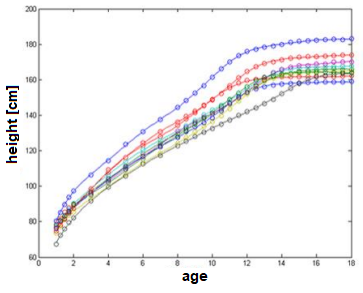
\includegraphics[width=10.5 cm]{images/berkeley}
\caption{Sample curves of functional data - height of girls during their growing, based on \href{https://www.jstor.org/stable/1125347}{Berkeley growth study}.}
\end{figure}
\unskip

\vspace{5mm}
Functional version of logistic regression takes many assumptions and similarities from classical approach as other FDA concepts. The sigmoid function (6) stays the same, but with continuous independent variable $ x(t) $ and coefficient function $ \beta(t)$. Thus, the following form of conditional success probability can be expressed as
\begin{linenomath}
\begin{equation}
\pi(x) = \frac{e^{\alpha + \int_T \beta(t)x(t)dt}}{1 + e^{\alpha + \int_T \beta(t)x(t)dt}},
\end{equation}
\end{linenomath}
where $\alpha$ is a bias or intercept parameter and $\beta(t)$, instead of a vector, is a coefficient function square-integrable on $T$. Thus, defined predictor $\pi(x)$ takes independent variables $X : T$ and returns the calculated probability. The same assumptions can be used while describing the multiclass variant as well. 

The main goals of functional logistic regression, especially in use with time series, are classification purposes, prediction of new responses and estimation of $\beta$ function. Of course practical observations must be discrete due to physical limitations, but the subjects $x_1, x_2, ..., x_k$ are considered as functions. To handle the high dimension of collected data and preserve its functional nature, it is common to use a basis expansions, such as a B-spline basis, a Fourier basis or a wavelet basis \cite{logreg-comparison}. 

If bases for expansion are selected as $\theta$ for sampling trajectory and $\omega$ for coefficient function, these functions can be described as
\begin{linenomath}
\begin{equation}
x_i(t) = \sum_{k=1}^{K_x} c_{ik} \theta_k (t) = {\bf c}_i^T \theta (t),
\hspace{5mm} \beta(t) = \sum_{l=1}^{K_{\beta}} b_l \omega_l (t) = \omega^T (t) {\bf b},
\end{equation}
\end{linenomath}
where $\theta_k (t)$ and $\omega_l (t)$ represent the $k$th and $l$th basis functions evaluated at time $t$.

%%%%%%%%%%%%%%%%%%%%%%%%%%%%%%%%%%%%%%%%%%
\subsection{Universal motor audio recording case study}

%%%%%%%%%%%%%%%%%%%%%%%%%%%%%%%%%%%%%%%%%%
\section{Results}

\subsection{Computational setup}

The practical implementation of functional logistic regression in binary variant is based on and developed from Python library for functional data analysis \href{https://fda.readthedocs.io/en/latest/index.html}{scikit-fda}. The multiclass variant is made from scratch, based on the same library as well as solutions for classical approaches stored in \href{https://scikit-learn.org/}{scikit-learn} library. The final proposed implementation is stored as a public, open-source \href{https://github.com/Porbi96/fda-time-series-classification}{GitHub repository}. The repository contains also a demonstration with use of mock data and practical use based on data possessed.

The database used for practical tests and visualizations contains voice recordings of commutator motors both damaged and undamaged. More information about the data can be found in \cite{ref-motors}.

%%%%%%%%%%%%%%%%%%%%%%%%%%%%%%%%%%%%%%%%%%

\subsection{Common preprocessing}

The process flow is prepared for existing dataset of voice recordings, but can be easily changed to cover other issues. The flow starts with loading the data as a discrete time series of samples recorded, which is then transformed by Fourier transformation and normalized to the form of discrete function of frequency, where values are in between 0 and 1. The frequency range is limited by the voice recording device and in this case covers half of sample rate, which is 44100Hz, due to aliasing issues.

\vspace{5mm}
TODO: the preprocessing flow diagram or list can be put.
\vspace{5mm}

\subsection{Binary variant}

For binary variant, any two of given labels can be used. In the demo, recordings of two groups of damaged motors are chosen: ones with two damaged teeth and ones with five damaged teeth. 

\vspace{5mm}
TODO: put graph of raw data after Fourier transformation for the groups chosen in demo.
\vspace{5mm}

Such prepared data is then transformed into functional dataset by use of basis spline data interpolation. In the example, 45 basis functions of 4th order is used. The values are found experimentally and might strongly depend on analyzed data. Due to dataset limitations of 30 recordings per group, 60 separate functions are prepared.

\vspace{5mm}
TODO: put graph of functional data.
\vspace{5mm}

Ready to be use functional data is then used in a binary functional logistic regression model fitting process, which is analogous to classical discrete version known for example in machine learning algorithms. The dataset is split into training and validation subsets. Thereafter the model is taught on training data, trying to fit coefficients to gain best accuracy. Final model score is obtained on validation subset, which is unknown to model during the fitting process.

For the dataset of two groups of motors model accuracy is up to 88 percent. The result depends on the dataset splitting method a lot, due to small size of the dataset. Populating data could increase the model stability. 

\vspace{5mm}
TODO: put graph of functional data after classification.
\vspace{5mm}

\subsection{Multiclass variant}

The multiclass variant is suitable for three or more labels. Implementation is tested on three separate classes of motor damage, containing 30 voice recordings each.

\vspace{5mm}
TODO: put graph of raw data after Fourier transformation for the groups chosen in demo.
\vspace{5mm}

The way data is transformed into functional basis spline functions remains the same as in binary variant. Due to choose of three classes, 90 functions are created, each containing info about different voice recording. 

\vspace{5mm}
TODO: put graph of functional data.
\vspace{5mm}

Prepared and labeled data is used in multiclass functional logistic regression model in similar way as in the binary variant, so the dataset is once again split into training and validation subsets in the same proportion. Model after fitting process gains around 77 percent of accuracy when tested on validation subset. The result is again depend on the splitting method due to small size of dataset.

\vspace{5mm}
TODO: put graph of functional data after classification.
\vspace{5mm}


% This section may be divided by subheadings. It should provide a concise and precise description of the experimental results, their interpretation as well as the experimental conclusions that can be drawn.
% \subsection{Subsection}
% \subsubsection{Subsubsection}

% Bulleted lists look like this:
% \begin{itemize}
% \item	First bullet;
% \item	Second bullet;
% \item	Third bullet.
% \end{itemize}

% Numbered lists can be added as follows:
% \begin{enumerate}
% \item	First item; 
% \item	Second item;
% \item	Third item.
% \end{enumerate}

% The text continues here. 

% \subsection{Figures, Tables and Schemes}

% All figures and tables should be cited in the main text as Figure~\ref{fig1}, Table~\ref{tab1}, Table~\ref{tab2}, etc.

% \begin{figure}[H]
% 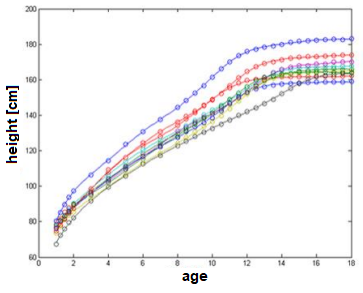
\includegraphics[width=10.5 cm]{images/berkeley}
% \caption{This is a figure. Schemes follow the same formatting. If there are multiple panels, they should be listed as: (\textbf{a}) Description of what is contained in the first panel. (\textbf{b}) Description of what is contained in the second panel. Figures should be placed in the main text near to the first time they are cited. A caption on a single line should be centered.\label{fig1}}
% \end{figure}   
% \unskip

% \begin{table}[H] 
% \caption{This is a table caption. Tables should be placed in the main text near to the first time they are~cited.\label{tab1}}
% \newcolumntype{C}{>{\centering\arraybackslash}X}
% \begin{tabularx}{\textwidth}{CCC}
% \toprule
% \textbf{Title 1}	& \textbf{Title 2}	& \textbf{Title 3}\\
% \midrule
% Entry 1		& Data			& Data\\
% Entry 2		& Data			& Data\\
% \bottomrule
% \end{tabularx}
% \end{table}
% \unskip

% \begin{table}[H]
% \caption{This is a wide table.\label{tab2}}
% 	\begin{adjustwidth}{-\extralength}{0cm}
% 		\newcolumntype{C}{>{\centering\arraybackslash}X}
% 		\begin{tabularx}{\fulllength}{CCCC}
% 			\toprule
% 			\textbf{Title 1}	& \textbf{Title 2}	& \textbf{Title 3}     & \textbf{Title 4}\\
% 			\midrule
% 			Entry 1		& Data			& Data			& Data\\
% 			Entry 2		& Data			& Data			& Data \textsuperscript{1}\\
% 			\bottomrule
% 		\end{tabularx}
% 	\end{adjustwidth}
% 	\noindent{\footnotesize{\textsuperscript{1} This is a table footnote.}}
% \end{table}

% %\begin{listing}[H]
% %\caption{Title of the listing}
% %\rule{\columnwidth}{1pt}
% %\raggedright Text of the listing. In font size footnotesize, small, or normalsize. Preferred format: left aligned and single spaced. Preferred border format: top border line and bottom border line.
% %\rule{\columnwidth}{1pt}
% %\end{listing}

% Text.

% Text.

% \subsection{Formatting of Mathematical Components}

% This is the example 1 of equation:
% \begin{linenomath}
% \begin{equation}
% a = 1,
% \end{equation}
% \end{linenomath}
% the text following an equation need not be a new paragraph. Please punctuate equations as regular text.
% %% If the documentclass option "submit" is chosen, please insert a blank line before and after any math environment (equation and eqnarray environments). This ensures correct linenumbering. The blank line should be removed when the documentclass option is changed to "accept" because the text following an equation should not be a new paragraph.

% This is the example 2 of equation:
% \begin{adjustwidth}{-\extralength}{0cm}
% \begin{equation}
% a = b + c + d + e + f + g + h + i + j + k + l + m + n + o + p + q + r + s + t + u + v + w + x + y + z
% \end{equation}
% \end{adjustwidth}

% % Example of a page in landscape format (with table and table footnote).
% %\startlandscape
% %\begin{table}[H] %% Table in wide page
% %\caption{This is a very wide table.\label{tab3}}
% %	\begin{tabularx}{\textwidth}{CCCC}
% %		\toprule
% %		\textbf{Title 1}	& \textbf{Title 2}	& \textbf{Title 3}	& \textbf{Title 4}\\
% %		\midrule
% %		Entry 1		& Data			& Data			& This cell has some longer content that runs over two lines.\\
% %		Entry 2		& Data			& Data			& Data\textsuperscript{1}\\
% %		\bottomrule
% %	\end{tabularx}
% %	\begin{adjustwidth}{+\extralength}{0cm}
% %		\noindent\footnotesize{\textsuperscript{1} This is a table footnote.}
% %	\end{adjustwidth}
% %\end{table}
% %\finishlandscape

% % Example of a figure that spans the whole page width. The same concept works for tables, too.
% \begin{figure}[H]
% \begin{adjustwidth}{-\extralength}{0cm}
% \centering
% 
\includegraphics[width=13.5cm]{Definitions/logo-mdpi}
% \end{adjustwidth}
% \caption{This is a wide figure.\label{fig2}}
% \end{figure}  

% Please punctuate equations as regular text. Theorem-type environments (including propositions, lemmas, corollaries etc.) can be formatted as follows:
% %% Example of a theorem:
% \begin{Theorem}
% Example text of a theorem.
% \end{Theorem}

% The text continues here. Proofs must be formatted as follows:

% %% Example of a proof:
% \begin{proof}[Proof of Theorem 1]
% Text of the proof. Note that the phrase ``of Theorem 1'' is optional if it is clear which theorem is being referred to.
% \end{proof}
% The text continues here.

%%%%%%%%%%%%%%%%%%%%%%%%%%%%%%%%%%%%%%%%%%
\section{Discussion}

Authors should discuss the results and how they can be interpreted from the perspective of previous studies and of the working hypotheses. The findings and their implications should be discussed in the broadest context possible. Future research directions may also be highlighted.

%%%%%%%%%%%%%%%%%%%%%%%%%%%%%%%%%%%%%%%%%%
\section{Conclusions}

This section is not mandatory, but can be added to the manuscript if the discussion is unusually long or complex.

%%%%%%%%%%%%%%%%%%%%%%%%%%%%%%%%%%%%%%%%%%
\vspace{6pt} 

%%%%%%%%%%%%%%%%%%%%%%%%%%%%%%%%%%%%%%%%%%
%% optional
%\supplementary{The following supporting information can be downloaded at:  \linksupplementary{s1}, Figure S1: title; Table S1: title; Video S1: title.}

% Only for the journal Methods and Protocols:
% If you wish to submit a video article, please do so with any other supplementary material.
% \supplementary{The following supporting information can be downloaded at: \linksupplementary{s1}, Figure S1: title; Table S1: title; Video S1: title. A supporting video article is available at doi: link.}

%%%%%%%%%%%%%%%%%%%%%%%%%%%%%%%%%%%%%%%%%%
\authorcontributions{For research articles with several authors, a short paragraph specifying their individual contributions must be provided. The following statements should be used ``Conceptualization, J.B. ; methodology, J.B.; software, J.P.; validation, J.P. and J.B.; formal analysis, J.P. and J.B; investigation, J.P.; resources, J.B.; data curation, J.P.; writing---original draft preparation, J.P.; writing---review and editing, J.P. and J.B.; visualization, J.P.; supervision, J.B.; project administration, J.B.; funding acquisition, J.B. All authors have read and agreed to the published version of the manuscript.}

\funding{This research was funded by AGH’s Research University Excellence Initiative under project “Interpretable methods of process diagnosis using statistics and machine learning” and by Polish National Science Centre project “Process Fault Prediction and Detection” contract no. UMO-2021/41/B/ST7/03851}

\institutionalreview{Not applicable.}

\informedconsent{Not applicable.}

\dataavailability{{\color{red}TODO}} 

\acknowledgments{Authors would like express their gratitude to Prof. Adam Głowacz for providing data and Prof. Edyta Kucharska for administrative support}

\conflictsofinterest{The authors declare no conflict of interest.} 

%%%%%%%%%%%%%%%%%%%%%%%%%%%%%%%%%%%%%%%%%%


%% Only for journal Encyclopedia
%\entrylink{The Link to this entry published on the encyclopedia platform.}

\abbreviations{Abbreviations}{
The following abbreviations are used in this manuscript:\\

\noindent 
\begin{tabular}{@{}ll}
FDA & Functional Data Analysis\\
 & \\
 & \\
 & 
\end{tabular}
}



%%%%%%%%%%%%%%%%%%%%%%%%%%%%%%%%%%%%%%%%%%
\begin{adjustwidth}{-\extralength}{0cm}
%\printendnotes[custom] % Un-comment to print a list of endnotes

\reftitle{References}

% Please provide either the correct journal abbreviation (e.g. according to the “List of Title Word Abbreviations” http://www.issn.org/services/online-services/access-to-the-ltwa/) or the full name of the journal.
% Citations and References in Supplementary files are permitted provided that they also appear in the reference list here. 

%=====================================
% References, variant A: external bibliography
%=====================================
\bibliography{bibliography.bib}

%=====================================
% References, variant B: internal bibliography
%=====================================
% \begin{thebibliography}{999}

% \end{thebibliography}

% If authors have biography, please use the format below
%\section*{Short Biography of Authors}
%\bio
%{\raisebox{-0.35cm}{\includegraphics[width=3.5cm,height=5.3cm,clip,keepaspectratio]{Definitions/author1.pdf}}}
%{\textbf{Firstname Lastname} Biography of first author}
%
%\bio
%{\raisebox{-0.35cm}{\includegraphics[width=3.5cm,height=5.3cm,clip,keepaspectratio]{Definitions/author2.jpg}}}
%{\textbf{Firstname Lastname} Biography of second author}

% For the MDPI journals use author-date citation, please follow the formatting guidelines on http://www.mdpi.com/authors/references
% To cite two works by the same author: \citeauthor{ref-journal-1a} (\citeyear{ref-journal-1a}, \citeyear{ref-journal-1b}). This produces: Whittaker (1967, 1975)
% To cite two works by the same author with specific pages: \citeauthor{ref-journal-3a} (\citeyear{ref-journal-3a}, p. 328; \citeyear{ref-journal-3b}, p.475). This produces: Wong (1999, p. 328; 2000, p. 475)

%%%%%%%%%%%%%%%%%%%%%%%%%%%%%%%%%%%%%%%%%%
%% for journal Sci
%\reviewreports{\\
%Reviewer 1 comments and authors’ response\\
%Reviewer 2 comments and authors’ response\\
%Reviewer 3 comments and authors’ response
%}
%%%%%%%%%%%%%%%%%%%%%%%%%%%%%%%%%%%%%%%%%%
\end{adjustwidth}
\end{document}

